\documentclass[11pt]{article}
\usepackage[margin=2.6cm]{geometry}
\usepackage{mathpazo}
\usepackage{amsmath}
\usepackage{microtype}
\usepackage{booktabs}
\usepackage{array}
\usepackage{tikz}
\usepackage[font=small,labelfont=bf]{caption}
\usepackage{titlesec}
\titleformat{\section}{\large\bfseries}{\thesection}{0.8em}{}
\titleformat{\subsection}{\normalsize\bfseries\itshape}{\thesubsection}{0.8em}{}
\setlength{\parskip}{0.55em}
\setlength{\parindent}{0pt}
\begin{document}

\begin{center}
{\LARGE\bfseries What the Policy Sees}\\[0.5em]
{\large Observation of the CALM speed recommender}
\end{center}
\vspace{0.6em}

\section{When the policy observes}

The policy decides once per bump. The observation it receives is taken at the moment the slowdown window opens, $25$\,m before the bump, while the car is still cruising at about the scenario speed. Everything the policy needs to choose a depth must therefore be in this one vector: how the car is moving, and what the road ahead looks like.

\section{Layout}

The observation has $23$ numbers: $8$ describe the vehicle and $15$ describe the road ahead (Table~\ref{tab:obs}).

\begin{table}[h]
\centering
\renewcommand{\arraystretch}{1.25}
\begin{tabular}{@{}r p{5.3cm} p{6.4cm}@{}}
\toprule
No. & Quantity & Definition \\
\midrule
\multicolumn{3}{@{}l}{\textit{Vehicle (8)}}\\
1 & Front wheel travel & front wheel height minus body height (m) \\
2 & Wheel acceleration & vertical acceleration of the wheel (m/s$^2$) \\
3 & Body acceleration & vertical acceleration of the body (m/s$^2$) \\
4 & Pitch acceleration & angular acceleration of the pitch (rad/s$^2$) \\
5 & Pitch angle & body pitch (rad) \\
6 & Speed & current speed $v$ (m/s) \\
7 & Longitudinal acceleration & acceleration of the last step (m/s$^2$) \\
8 & Speed error & reference speed minus current speed (m/s) \\
\midrule
\multicolumn{3}{@{}l}{\textit{Road ahead (15)}}\\
9--12 & Nearest bump ahead & distance, width, height, frequency (see below) \\
13--16 & Second bump ahead & same four values \\
17--20 & Third bump ahead & same four values \\
21 & Speed ratio & $v / v_{\mathrm{top}}$ \\
22 & Distance since last bump & distance to the end of the last bump passed, divided by $40$\,m \\
23 & On-bump flag & $1$ while a bump is under the car, else $0$ \\
\bottomrule
\end{tabular}
\caption{The 23 observed values.}\label{tab:obs}
\end{table}

\section{Road ahead}

The preview looks $D = 40$\,m ahead (Figure~\ref{fig:preview}) and lists the bumps whose start lies within this distance and whose end the car has not yet passed, nearest first, at most three. Holes are not listed. For a bump with start distance $d$, width $L$ and height $A$ the four values are scaled to $[0,1]$:
\begin{equation}
\frac{d}{40\,\mathrm{m}}, \qquad \frac{L}{8\,\mathrm{m}}, \qquad \frac{A}{0.15\,\mathrm{m}}, \qquad \frac{v_{\mathrm{top}}/L}{10\ \mathrm{Hz}},
\end{equation}
each clipped to $[0,1]$. The last value is the frequency at which the wheel meets the bump at the top speed $v_{\mathrm{top}}$, the larger of the scenario speed and the speed floor; it is the quantity that decides whether the bump excites the body or the wheel. A bump that is not present is filled with $(1,0,0,0)$: far away, no width, no height, no excitation. The speed ratio is $v/v_{\mathrm{top}}$ and the distance since the last bump is set to $1$ when no bump has been passed.

\begin{figure}[h]
\centering
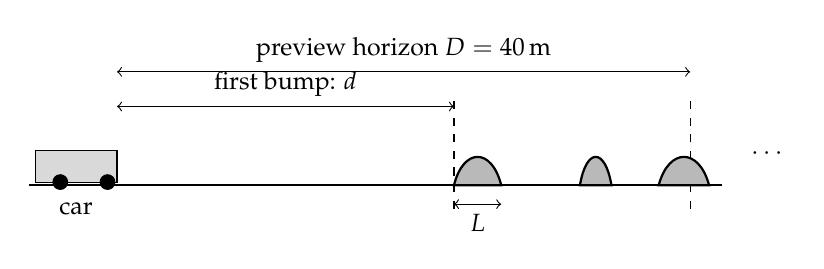
\begin{tikzpicture}[x=0.2cm, y=0.2cm]
\draw[thick] (-2,0) -- (42,0);
\fill[gray!30] (-1.6,0.2) rectangle (3.6,2.2);
\draw (-1.6,0.2) rectangle (3.6,2.2);
\fill (0,0.2) circle (0.5); \fill (3,0.2) circle (0.5);
\node[below] at (1,-0.5) {\small car};
\draw[thick] (-2,0) -- (4,0);
\draw[dashed] (25,-1.5) -- (25,5.8);
\draw[dashed] (40,-1.5) -- (40,5.8);
\draw[<->] (3.6,5) -- (25,5) node[midway, above] {\small first bump: $d$};
\draw[<->] (3.6,7.2) -- (40,7.2) node[midway, above] {\small preview horizon $D = 40$\,m};
\foreach \x/\w in {25/3, 33/2, 38/3.2}{
  \draw[thick, fill=gray!55] (\x,0) .. controls (\x+0.2*\w,2.4) and (\x+0.8*\w,2.4) .. (\x+\w,0) -- cycle;
}
\draw[<->] (25,-1.2) -- (28,-1.2) node[midway, below] {\small $L$};
\node[font=\small] at (45,2) {$\cdots$};
\end{tikzpicture}
\caption{Geometry of the preview. Bumps beyond $D$ are not visible.}\label{fig:preview}
\end{figure}

\section{Perception}

The baseline observes the true bump geometry of the road: no noise is added and no camera detector is in the loop. The policy is therefore trained and scored as if the road ahead were detected perfectly. A camera-based detector with measured range bias and noise exists as a separate option of the environment (replay of recorded detections, or a noise model fitted to them); it is not used in the baseline.

\section{Normalisation}

During training the observation is normalised with a running mean and standard deviation per value and clipped to $\pm 10$. The statistics are saved with the policy in \texttt{vecnormalize.pkl}; the policy cannot be used without them.

\section{Limits}

The policy sees at most three bumps within $40$\,m, so a bump farther away does not influence the decision. Because the observation is taken when the window opens, the vehicle values carry little information; most of the decision rests on the preview of the next bump and the scenario speed.

\end{document}
